\section {Etapa de escritura}

En esta etapa se ponen en marcha la escritura de registros si es que esa bandera esta habilitada, en otro caso no es una etapa imprescindible, pero es necesaria para algunas instrucciones.

\begin{figure}[H]
\centering
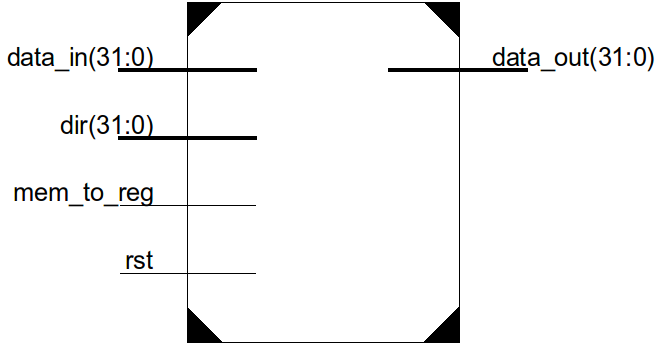
\includegraphics[scale=0.5]{img/wb_stage}
\caption{Etapa de Escritura}
\label{fig:wb_stage}
\end{figure}

Tiene como entradas:
\begin{itemize}
  \item \textbf{data\_in}: Bus de 32 bits que contiene el dato que se obtiene de la memoria.
  \item \textbf{dir}: Datos que se van a escribir en el banco de registros.
  \item \textbf{mem\_to\_reg}: Señal que activa el multiplexor dentro de la etapa y elige entre data\_in y dir.
  \item \textbf{rst}: Reset general del m\'odulo.
\end{itemize}

Salidas:
\begin{itemize}
  \item \textbf{data\_out}: Dato de salida seg\'un la elecci\'on del multiplexor.
\end{itemize}